%  Paper in preparation for submission to Sensors for the special issue "Application of Unmanned Aircraft Systems for Atmospheric Science"
%=================================================================
\documentclass[sensors,review,submit,moreauthors,pdftex,10pt,a4paper]{mdpi} 
%=================================================================
\firstpage{1} 
\makeatletter 
\setcounter{page}{\@firstpage} 
\makeatother 
\articlenumber{x}
\doinum{10.3390/------}
\pubvolume{xx}
\pubyear{2018}
\copyrightyear{2018}
\externaleditor{Academic Editor: name}
\history{Received: date; Accepted: date; Published: date}
%------------------------------------------------------------------
% The following line should be uncommented if the LaTeX file is uploaded to arXiv.org
%\pdfoutput=1

%=================================================================
% Add packages and commands here. The following packages are loaded in our class file: fontenc, calc, indentfirst, fancyhdr, graphicx, lastpage, ifthen, lineno, float, amsmath, setspace, enumitem, mathpazo, booktabs, titlesec, etoolbox, amsthm, hyphenat, natbib, hyperref, footmisc, geometry, caption, url, mdframed

%=================================================================
%% Please use the following mathematics environments:
 \theoremstyle{mdpi}
 \newcounter{thm}
 \setcounter{thm}{0}
 \newcounter{ex}
 \setcounter{ex}{0}
 \newcounter{re}
 \setcounter{re}{0}

 \newtheorem{Theorem}[thm]{Theorem}
 \newtheorem{Lemma}[thm]{Lemma}
 \newtheorem{Corollary}[thm]{Corollary}
 \newtheorem{Proposition}[thm]{Proposition}

 \theoremstyle{mdpidefinition}
 \newtheorem{Characterization}[thm]{Characterization}
 \newtheorem{Property}[thm]{Property}
 \newtheorem{Problem}[thm]{Problem}
 \newtheorem{Example}[ex]{Example}
 \newtheorem{ExamplesandDefinitions}[ex]{Examples and Definitions}
 \newtheorem{Remark}[re]{Remark}
 \newtheorem{Definition}[thm]{Definition}
%% For proofs, please use the proof environment (the amsthm package is loaded by the MDPI class).

%=================================================================
% Full title of the paper (Capitalized)
\Title{Moving Towards a Network of Autonomous UAS Atmospheric Profiling Stations for Observations in the Earth’s Lower Atmosphere: The 3D Mesonet Concept}

% Authors, for the paper (add full first names)
\Author{Phillip B. Chilson $^{1,\dagger,\ddagger}$,
Fred Carr$^{1}$,
Christopher Fiebrich $^{1,\ddagger}$,
Mark Yeary$^{1}$,
Robert Huck$^{1}$,
Keith Brewster$^{1}$,
Elizabeth Pillar-Little$^{1}$,
Robert D. Palmer$^{1}$,
Mark Weber$^{1}$,
Kenneth Carson$^{1}$,
Jorge Salazar-Cerreno$^{1}$,
Brian Greene$^{1}$,
Tyler Bell$^{1}$,
Antonio R. Segales$^{1}$,
Gustavo Britto Hupsel de Azevedo$^{1}$,
Sai Teja Kanneganti$^{1}$,
William Doyle$^{1}$,
James Grimsley$^{1}$,
Joshua Martin$^{1}$,
Brent Wolf$^{1}$,
and
Kelvin Droegemeier$^{1}$,
}
% Authors, for metadata in PDF
\AuthorNames{Phillip B. Chilson, Firstname Lastname and Firstname Lastname}

% Affiliations / Addresses (Add [1] after \address if there is only one affiliation.)
\address{%
$^{1}$ \quad Affiliation 1; e-mail@e-mail.com\\
$^{2}$ \quad Affiliation 2; e-mail@e-mail.com}

% Contact information of the corresponding author
\corres{Correspondence: chilson@ou.edu; Tel.: +1-405-325-5095}

% Current address and/or shared authorship
\firstnote{Current address: Affiliation 3} 
\secondnote{These authors contributed equally to this work.}

% Simple summary
%\simplesumm{}

% Abstract (Do not use inserted blank lines, i.e. \\) 
\abstract{The deployment of small unmanned aircraft to collect in-situ vertical measurements of the atmospheric state in conjunction with other meteorological observations has the potential to significantly expand our weather observation capabilities. We briefly report on a concept of adding the capability of collecting vertical atmospheric measurements (profiles) through the use of unmanned aerial systems (UAS) at sites deemed suitable for this application.  The system must be able to operate unattended, which necessitates the inclusion of risk mitigation measures such as detect and avoid radar and the ability to transmit and receive transponder signals. It is also necessary for the system to be capable of assessing local weather conditions (visibility, surface winds, cloud height) and the integrity of the vehicle (system diagnostics, fuel level) before takeoff. We begin by providing a notional concept of operations for a 3D Mesonet and a description of the technical configuration for one such station in the network. We then report on progress being made to develop and test a prototype 3D Mesonet station and show preliminary measurements and discuss how such measurements from an operational network could be utilized to better characterize the atmospheric boundary layer, improve weather forecasts, and help to identify threats of severe weather.}

% Keywords
\keyword{keyword 1; keyword 2; keyword 3. List three to ten pertinent keywords specific to the article, yet reasonably common within the subject discipline.}

% The fields PACS, MSC, and JEL may be left empty or commented out if not applicable
%\PACS{J0101}
%\MSC{}
%\JEL{}

% If this is an expanded version of a conference paper, please cite it here: enter the full citation of your conference paper, and add $^\S$ in the end of the title of this article.
%\conference{}

%%%%%%%%%%%%%%%%%%%%%%%%%%%%%%%%%%%%%%%%%%
% Only for the journal Data:

%\dataset{DOI number or link to the deposited data set in cases where the data set is published or set to be published separately. If the data set is submitted and will be published as a supplement to this paper in the journal Data, this field will be filled by the editors of the journal. In this case, please make sure to submit the data set as a supplement when entering your manuscript into our manuscript editorial system.}

%\datasetlicense{license under which the data set is made available (CC0, CC-BY, CC-BY-SA, CC-BY-NC, etc.)}

%%%%%%%%%%%%%%%%%%%%%%%%%%%%%%%%%%%%%%%%%%
\begin{document}

%%%%%%%%%%%%%%%%%%%%%%%%%%%%%%%%%%%%%%%%%%
%% Sections that are not mandatory are listed as such. The section titles given are for Articles. Review papers and other article types have a more flexible structure. 

%% Only for the journal Gels: Please place the Experimental Section after the Conclusions

%%%%%%%%%%%%%%%%%%%%%%%%%%%%%%%%%%%%%%%%%%%%%%%%%%%%%%%%%%%%%%%%%%%%%%%%%%%%%%%%%%%%%%%%%%%%%
\section{Introduction}
%%%%%%%%%%%%%%%%%%%%%%%%%%%%%%%%%%%%%%%%%%%%%%%%%%%%%%%%%%%%%%%%%%%%%%%%%%%%%%%%%%%%%%%%%%%%%
\begin{itemize}[leftmargin=*,labelsep=4mm]
\color{blue}
\item	Discuss the complexity of the atmospheric boundary layer (ABL) and the importance of monitoring and modeling this region
\item	Difficulty in acquiring adequate and quality measurements with conventional instrumentation in the ABL
\item	Provide a graphic of the ABL (Figure \ref{fig:ABLCartoon})
\item	Recommendations from NAS, NRC, NCAR, NSF, etc to collect more data in the ABL
\item	Growing development of UAS for atmospheric measurements and how this could fill the measurement gap
\item	Briefly introduce the 3D Mesonet Concept
\item	How these observations could impact weather forecasting and more
\item	Layout the paper structure
\end{itemize}

Dramatic, high-impact weather events, such as severe thunderstorms with hail and wind, tornadoes, excessive rainfall and flooding, tropical storms, ice storms, heavy snowstorms, and blizzards have an impact of billions of dollars per year on the economy of the United States \citep{lazo++2011_BAMS, bloesch+2015_EconPerspectives}. Additionally, a number of industries in the US are quite weather sensitive, including agriculture, transportation and electric power generation and management. Definitive links are being made between climate change and the impact it is having on the occurrence of dramatic weather events \citep{wmo2018}. To mitigate deleterious impacts on society and its infrastructure, it is imperative that we develop innovative means of monitoring and modeling the Earth's atmosphere. To achieve this end, we require better observations of the lower atmosphere and an effective means of incorporating these measurements into numerical weather predictions. That  is, the availability of quality atmospheric observations is critical to our ability to monitor meteorological conditions and accurately forecast the weather.

Meteorological observations fall largely into two categories: in-situ and remote sensing. The former involves the measurement by instruments, which are directly exposed to the atmosphere. In this case, continual observations of the atmosphere are limited to sensors, which can be placed at or near the Earth's surface (e.g., using instrumented towers). To obtain in-situ measurements aloft, balloons, kites, or aircraft must be used. Sensors capable of remotely probing the Earth's atmosphere, such as radar, are capable of providing continual observation. However, the number of atmospheric parameters such technologies can provide is limited and the data often must be inferred from other measured quantities (e.g., radar reflectivity).  For example, rainfall rates provided by weather radar are estimated based on the strength of the backscattered signal from the precipitation.

A long-desired component to the U.S. operational observing systems is the capability to measure vertical profiles of wind, temperature and moisture in the lower troposphere at high spatial and temporal resolution. Sounding data can be used to assess regions of thermal stratification and the degree of atmospheric static and dynamic stability. Overall, processes in the PBL can vary dramatically over a single diurnal cycle as depicted in Figure~\ref{fig:ABLCartoon}. Although this conceptual model of the PBL is idealized, it helps to illuminate several common features of the PBL structure: mixed layer, capping and nocturnal inversion, the surface layer, the residual layer, and so forth. To fully characterize the PBL, measurements of the state parameters in each of these regions are needed, preferably with adequate temporal resolution to fully capture evolution of the height of the PBL and structures within the PBL.

% *******************************************************************************************
\begin{figure}
\centering
\includegraphics[angle=0, width=\textwidth]{figures/ABL_profiles_cartoon.pdf}
\caption{\label{fig:ABLCartoon} Schematic depicting the idealized structure of the PBL (left) during one diurnal cycle under quiescent conditions. Vertical profiles of the temperature at five particular times (denoted as A-E) are presented to the right. In this cloud-free example, the structure of the PBL is primarily driven by thermal forcing produced by insolation. \textcolor{red}{Modify figure or use Tyler's figure.}}
\end{figure}
% *******************************************************************************************

This need is reflected in several recent studies, some of which provide explicit recommendations to collect more observations within the atmospheric boundary layer (ABL), in general with a focus on vertical sampling (profiling) in particular \citep{NRC2009, hardesty+2012, 2017_2027_DecadalSurvey, NAP25138, geerts++2017_UCAR}. These reports emphatically state that our currently available observing systems are not capable of providing adequately detailed profiles of temperature, moisture, and winds within the ABL. Height profiles of virtual potential temperature can be used to identify regions of thermal stratification and the degree of atmospheric stability. Moreover, vertical wind shear is capable of producing turbulence and thus turbulent fluxes in the ABL. Overall, processes in the ABL can vary dramatically over a single diurnal cycle. A depiction of the structure of the ABL during a typical diurnal cycle is provided in Figure~\ref{fig:ABLCartoon}.

To address these considerations, advance several key recommendations listed in the NASA Science Plan, and fulfill the mandates put before NOAA in the 2017 Weather Research Innovation Act, we must challenge ourselves to develop observing and modeling systems that transcend the conventional methods. An emerging technology, which could have dramatic impacts on observations of the lower atmosphere, is that of Unmanned Aircraft Systems (UAS). It has been suggested that such profiling could be done by small unmanned aerial vehicles (UAVs) assuming that autonomous flights extend at least through the depth of the boundary layer \citep{dabberdt++2005_BAMS}. As outlined below, instrumented UAS are expected to provide inexpensive, accurate, controlled, observations of the lower atmosphere. The advent of weather-observing UAS (WxUAS) would complement other observing systems, such as rawinsondes, towers, satellite-based remote sensors, and active and passive ground-based remote sensors. The true value of WxUAS lies in their ability to fill data gaps that conventional instrumentation cannot easily or feasibly provide, for example in the PBL.

\textcolor{red}{Reword this.} In recent decades, numerous states have established networks of \textit{in-situ} meteorological observing stations (i.e.,  Mesonets) to aid decision making across various sectors ranging from emergency management to agriculture to weather forecasting to transportation \citep{mahmood++2017_BAMS, ziolkowska++2017_WCAS}. In general, Mesonets aim to provide multi-purpose, high-quality, real-time observations. Additionally, they provide tailored outreach (typically to the K-12, university, public safety, and agriculture communities) to expand the utility of the observations. Across the United States, there are currently 27 statewide networks of mesoscale in situ meteorological observations (i.e., Mesonets; \cite{mahmood++2017_BAMS}). These networks range in size from less than 10 stations to over 175 stations, but each have a goal of providing high resolution observations to support mesoscale weather and climate monitoring. Typically, mesonets include sensors mounted on or below a 10 m tower to sample air temperature, relative humidity, winds, solar radiation, precipitation, pressure, and soil temperatures and soil moisture.

\textcolor{red}{Reword this and work in an introduction of the 3D Mesonet.} Typical Mesonet stations are located in areas that have minimal slope and minimal obstructions that impede environmental fetch. \citet{ziolkowska++2017_WCAS} documented the value of mesonet data to many diverse sectors across Oklahoma, including those in agriculture, drought and climate monitoring, public safety, wildland fire management, nowcasting, and energy management. Mesonet observations are increasingly being used in forecast model development and in understanding land-atmosphere interactions. Both \citet{mahmood++2017_BAMS} and \citet{ziolkowska++2017_WCAS} note that expanding Mesonet observations into the boundary layer via UAVs are an important next step to bring added value to sectors that could benefit from improved weather forecasts.

In addition to capturing the vertical structure of the PBL, WxUAS can be used to detect complex mesoscale features embedded in weather systems. In Figure~\ref{fig:OKMesoExample}, we present an example of the surface mesoscale wind and humidity field across Oklahoma on the afternoon of 26 March 2018. A combination of varying insolation across the state and the action of a cold front, dryline, and upper-level jet resulted in significant county-by-county variability. The implications of such features on wildfire risk (including likelihood for initiation, behavior, and smoke dispersion), convective initiation, and moisture and momentum fluxes are immense, yet inadequately understood without additional measurements of the PBL. It is difficult to understate the impact that additional mesoscale, 4D observations could have on detecting and predicting these phenomena.

As illustrated in Figure~\ref{fig:OKMesoExample}, the atmospheric surface layer can exhibit remarkably complex spatial structure in the wind and moisture fields. Moreover, the evolution of these structures over time can be equally complex. Even with observations from dense surface sensor networks, such as the Oklahoma Mesonet, the vertical structure remains unknown, so forecasters must rely on statistically-based parameterization schemes \citep{teixeira++2008_BAMS} and basic conceptual models to envision processes acting in the vertical dimension. Tremendous value would be added if the measurements depicted in Figure~\ref{fig:OKMesoExample} could be extended vertically through the depth of the PBL. Providing researchers and forecasters with data that allow them to monitor the changing 4D wind, temperature and moisture patterns would yield considerable benefits. For example, subtle changes in the strength of the capping inversion can have a profound impact on the probability of convective initiation and the chance that storms may become severe. Further, these data can be used to initialize mesoscale and thunderstorm-scale NWP. Knowing if, when, and where the cap might ``break'' is paramount to anticipating where convection could be initiated. Current parameterization schemes struggle to provide adequate information on the strength of the capping inversion, mostly due to lack of observational data.

% *******************************************************************************************
\begin{figure}
\centering
\includegraphics[angle=0, width=0.75\textwidth]{figures/OKMesoExample.pdf}
\caption{\label{fig:OKMesoExample} Mesonet station plot of relative humidity (\%) and wind field streamlines across Oklahoma during the afternoon of 26 March 2018.}
\end{figure}
% *******************************************************************************************

\textcolor{red}{Provide a layout of the paper}

%%%%%%%%%%%%%%%%%%%%%%%%%%%%%%%%%%%%%%%%%%%%%%%%%%%%%%%%%%%%%%%%%%%%%%%%%%%%%%%%%%%%%%%%%%%%%
\section{Overview of the 3D Mesonet Concept}
%%%%%%%%%%%%%%%%%%%%%%%%%%%%%%%%%%%%%%%%%%%%%%%%%%%%%%%%%%%%%%%%%%%%%%%%%%%%%%%%%%%%%%%%%%%%%

% ===========================================================================================
\subsection{Growth of WxUAS}
% ===========================================================================================
\begin{itemize}[leftmargin=*,labelsep=4mm]
\color{blue}
\item	Before launching into the 3D Mesonet, we provide a brief introduction to the growth and development of UAS for atmospheric measurements and weather observations (WxUAS)
\item	Discuss why we are currently witnessing growth in the area of UAS in general and WxUAS in particular
\item	Point out the growing interest in WxUAS as witnessed in professional societies: ISARRA and special sessions at AMS, AGU, AIAA
\item	WxUAS is transitioning from ``toys to tools''
\end{itemize}

There has been rapid development in WxUAS technology and its integration into meteorological research for atmospheric boundary layer studies (Reuder et al., 2009; Martin et al., 2011, Wildmann et al., 2014). Much of the initial studies with WxUAS were conducted using fixed-wing aircraft. An overview paper of these platforms can be found in Elston et al., 2015). More recently, rotary-wing vehicles are playing a prominent role in WxUAS research (e.g., Brosy et al., 2017; Hemingway et al., 2017; Lee et al., 2017). Overwhelmingly, the WxUAS presented in the current literature are one-off units developed by a research group for specific applications. 

Currently there are no small unmanned aircraft systems which offer all measurement and telemetry capabilities envisioned for autonomous operation. The proposed modular system will allow for customization, upgrade, and in-field replacement of sensor packages as desired. Such a system would facilitate off-site maintenance and calibration and would provide the ability to add new sensors as they are developed, or as new requirements are identified. The small WxUAS must be capable of handling the weight of all sensor packages and have lighting, communication, and aircraft avoidance systems necessary to meet existing or future FAA regulations. The system must be able to operate unattended or with remote piloting at such time that FAA regulations allow.

\textcolor{red}{Expand upon this and discuss how UAS is evolving from toy to tool.}

% ===========================================================================================
\subsection{Conceptual Framework of the 3D Mesonet}
% ===========================================================================================
\begin{itemize}[leftmargin=*,labelsep=4mm]
\color{blue}
\item	Pitch the 3D Mesonet concept
\item	Discuss how this might look when deployed across a broad footprint
\item	Provide a graphic of the 3D Mesonet concept (Figure \ref{fig:3DMesonetConcept})
\item	Need for unattended operations mandates:
\begin{itemize}[leftmargin=*,labelsep=4mm]
\item	Hardened UAVs with robust sensor units, which require minimal servicing and calibration;
\item	Detect and avoid radar unit
\item	ADS-B in \& out capability
\item	Ability to conduct internal diagnostics of the UAV and sensors
\item	Video monitoring
\item	Autonomous charging
\item	Two-way communications between UAV (with data feed) and a central control unit
\end{itemize}
\item	A prototype is being deployed at the Kessler Atmospheric and Ecological Field Station
\end{itemize}

\textcolor{red}{Introduce the Center for Autonomous Sensing and Sampling (CASS) in this disussion.}

The miniaturization and maturation of technology has progressed to the point where autonomous formations of small suborbital platforms, small Unmanned Aircraft Systems (sUAS), can be confidently deployed to collect spatiotemporal atmospheric measurements related to thermodynamic and kinematic state variables, particulate matter, and chemical components, which are critical to the understanding of planetary boundary layer (PBL) processes integral to air-surface (land, ocean and sea ice) exchanges of energy, momentum and mass; how these are affected by climate variability; and how they impact weather forecasts and air quality simulations. We assert that robust 4D datasets collected using instrumented sUAS together with appropriate modeling approaches will help address several of the most-important questions identified in the 2017-2027 Decadal Survey.

% *******************************************************************************************
\begin{figure}
\centering
\includegraphics[angle=0, width=\textwidth]{figures/3DMesonetConcept.pdf}
\caption{\label{fig:3DMesonetConcept} Placeholder: Graphic of the 3D Mesonet Concept. \textcolor{red}{Get original from Jorge or Arturo.}}
\end{figure}
% *******************************************************************************************

% ===========================================================================================
\subsection{Impact of Data on Weather Forecasting}
% ===========================================================================================
\begin{itemize}[leftmargin=*,labelsep=4mm]
\color{blue}
\item	Overview the philosophy \& use of Observation System Simulation Experiments
\item	Discuss how our OSSE was set up
\item	Provide some results (we need to hold back because Andrew will include this in his paper)
\end{itemize}

\textcolor{red}{Still stitching this together.} The PBL largely provides the moisture, instability, low-level wind shear, and forcing necessary for the formation of severe storms with attendant tornadoes, hail, and hazardous winds. Within the PBL resides the storm-generated outflows that can regulate the strength and longevity of severe storms or even trigger new storms. Knowledge of these conditions is the key to improving predictions of severe weather events. The problem is that PBL properties are highly variable on mesoscale time and space scales, which are virtually undetected by operational observing systems.

It has been well established that shear in the near-ground layer is critically important for distinguishing tornadic from nontornadic supercells and that traditional observational data, such as those provided by wind profiling radars do not provide adequate vertical resolution to resolve the shear \citep[e.g.,][]{markowski++1998_MWR}. The most noticeable difference between nontornadic and tornadic cases is in the lower-tropospheric wind profile; specifically the orientation of the 0-500~m shear vector with respect to the storm-relative inflow. This implies that the tornadic cases have much more streamwise horizontal vorticity in the lowest 500~m AGL \citep{coffer+2017_MWR}. Traditional standards used for radiosonde data processing do not capture features in the lowest 500~m well. Therefore, there is a need to sample the PBL near the surface with finer vertical resolution.

Since FAA permission has not yet been granted to test such an observing network, the potential improvement that a UAV network could have on storm-scale numerical weather prediction using an Observation System Simulation Experiment (OSSE) approach. An OSSE is performed over the state of Oklahoma in which it is assumed that a UAV could be launched from 110 Oklahoma Mesonet \citep{mcpheson++2007_JTECH} stations every hour, fly vertically to an assigned maximum altitude and return to its charging station, providing soundings at a roughly 35 km horizontal resolution. A case study of convective initiation (CI) was chosen for this study as a compromise between a fair-weather day and one with extensive ongoing convection. The OU ARPS \citep{xue++2000_MAP} model provides a nature run at high (1 km) resolution, while the control run and OSSE experiments are done with the WRF-ARW model at 3 km. To simulate the effect of data from dozens of observing systems already included in operational models, the nature run data volume is sampled at synoptic scales and inserted into the control run via a 6-hr data assimilation (DA) period. Simulated hourly UAV temperature, moisture and wind data, with expected errors, are then added to the DA, followed by 12-hr forecasts. The analyses and forecasts are examined to assess the added value of UAV data. Tests are run to measure the impact of varying the maximum UAV altitude and the spatial density of UAV observations.

Initial results clearly show an improved boundary layer structure and subsequent CI location and timing when UAV data are added to the control experiment. Through a series of experiments testing various maximum flight levels of the UAVs, it was determined that although flights up to 3 km above ground level (AGL) provided the best analysis of the boundary layer (Figure~\ref{fig:OSSE1}), flights up to 1 km were found to be sufficient in producing an improved CI forecast (Figure~\ref{fig:OSSE2}). On a similar note, a series of network density experiments found that while a UAV network consisting of 110 UAV stations produced the best results, the CI forecast was improved with only 75 UAV stations. Although sensitivities to the quality of the moisture analysis are noted, the results suggest that a real-world deployment of automated UAVs could have a positive impact on atmospheric analyses and short-term numerical weather prediction of convective initiation.

% *******************************************************************************************
\begin{figure}
\centering
\includegraphics[angle=0, width=0.75\textwidth]{figures/OSSE1.pdf}
\caption{\label{fig:OSSE1} \textcolor{red}{Need better figure from Moore} Cross section plots of mixing ratio for the Nature Run (A), WRF Control (B), No UAV (C), UAV 400ft (D), UAV 1km (E), UAV 2km (F), and UAV 3km (G) WRF analyses valid at 1800 UTC 20 May 2013. The Location of the cross section sample is depicted in the upper left image by the black line for reference.}
\end{figure}
% *******************************************************************************************

% *******************************************************************************************
\begin{figure}
\centering
\includegraphics[angle=0, width=0.75\textwidth]{figures/OSSE2.pdf}
\caption{\label{fig:OSSE2} \textcolor{red}{Need better figure from Moore}. Comparison between modeled composite radar reflectivity between the Nature Run (A), WRF Control (B), No UAV (C), UAV 400ft (D), UAV 1km (E), UAV 2km (F), and UAV 3km (G) at 1900 on 20 May 2013.}
\end{figure}
% *******************************************************************************************

%%%%%%%%%%%%%%%%%%%%%%%%%%%%%%%%%%%%%%%%%%%%%%%%%%%%%%%%%%%%%%%%%%%%%%%%%%%%%%%%%%%%%%%%%%%%%
\section{Platform and Sensor Development}
%%%%%%%%%%%%%%%%%%%%%%%%%%%%%%%%%%%%%%%%%%%%%%%%%%%%%%%%%%%%%%%%%%%%%%%%%%%%%%%%%%%%%%%%%%%%%
\begin{itemize}[leftmargin=*,labelsep=4mm]
\color{blue}
\item	Discuss the design criteria for the UAV
\item	Provide a discussion of the current version of the CopterSonde (will this material be discussed in another paper?)
\item	Include picture of the CopterSonde (Figure \ref{fig:CopterSondePic})
\item	Outline the specifications (Table 1)
\item	Mention the target accuracy for the sensors (Table 2)
\item	Refer to Greene et al.
\end{itemize}

The general concept of operations for the 3D Mesonet places certain design criteria on the WxUAS to be used. Flights should be conducted autonomously or semi-autonomously with minimal human interactions. It should consist of a vertical take-off and landing (VTOL) aircraft for the sake of docking and charging. This can be achieved using a rotary-wing aircraft or a hybrid vehicle capable of operating in a rotary-wing mode for take off and landing and then transitioning into a fixed-wing aircraft as its primary mode for data collection. Here we present developments rotary-wing VTOL vehicle using, known as the CopterSonde. Hybrid vehicles are currently under development within CASS and will be presented in forthcoming publications.

The CopterSonde series rotary-wing UAS was developed in-house by a CASS team of engineers and meteorologists to be both robust and optimized for atmospheric sampling. True to its name, the platforms are able to collect vertical profiles of the atmosphere like a traditional radiosonde or ozonesonde. However, these platforms provide highly resolved data (<10~m) in the lower atmosphere that are not easily achievable using conventional methods. The CopterSonde 2 (Figure~\ref{fig:CopterSondePic}) is based on the HQuad500 manufactured by Lynxmotion. It is comprised of carbon fiber plates, aluminum brackets, and carbon fiber tube legs. The rotary-wing craft is electrically powered by four identical brushless motors with T-style carbon fiber propellers. A lithium polymer battery pack with a capacity of 6750 mAh provides a maximum flight endurance of 25 minutes and can allow the platform to climb to a maximum altitude of 6000 ft ASL. The electronic components are protected from the elements with a custom 3D printed two-piece plastic shell, which was designed to enhance the vehicle's aerodynamics and allow for easy access to the interior components.

% *******************************************************************************************
\begin{figure}
\centering
\includegraphics[angle=0, width=0.75\textwidth]{figures/CopterSonde.pdf}
\caption{\label{fig:CopterSondePic} Placeholder: Picture of the CopterSonde}
\end{figure}
% *******************************************************************************************

All CopterSonde platforms utilize open-source technologies to enable autonomous operation of the vehicle. The first of these is a Pixhawk 2.1 flight controller (ProfiCNC), which is comprised of a rugged and vibrationally isolated microcontroller interfaced with a carrier board that allows for communication with a large variety of sensors over a wide range of communication protocols (I2C, UART, RS232, etc.) When paired with the Here+ GPS module (ProfiCNC), the Pixhawk is able to utilize Real Time Kinematic (RTK) GPS, which can reduce the uncertainty of the location of the UAS to less than 1 m in both the horizontal and vertical if properly set-up and calibrated. The microcontroller runs the ArduPilot autopilot software suite, which is composed of navigation software onboard the vehicle and ground station software that is transmitting commands to the UAS over telemetry link. When used with the flight controller, it creates a highly customizable environment that can be used to dictate the sampling speed of the sensors, flight path of the vehicle, ascent rate, and much more.

The CopterSonde 2 will be equipped with three Innovative Sensor Technology HYT 271 humidity sensors, three InterMet Bead Thermistors, and a MS5611 Barometer to measure pressure. The temperature and humidity sensors are located on the front of the vehicle in the 3D printed scoop designed to protect the sensors from solar radiation and serve as the front half of the platform's protective shell. A ducted fan is placed in the bottom of the scoop and used to aspirate the sensors by pulling air over them at a constant rate. The barometer is located inside of the autopilot. Wind velocity and direction is calculated using an ardupilot based algorithm that uses the pitch, yaw, and roll angle of the platform. Additionally, the rotary-wing craft uses the results of the wind algorithm to keep the vehicle facing into the wind as to allow for sampling of air undisturbed by the propellers. 

\textcolor{red}{Table of CopterSonde Specifications}


%%%%%%%%%%%%%%%%%%%%%%%%%%%%%%%%%%%%%%%%%%%%%%%%%%%%%%%%%%%%%%%%%%%%%%%%%%%%%%%%%%%%%%%%%%%%%
\section{Supporting Components of the 3D Mesonet}
%%%%%%%%%%%%%%%%%%%%%%%%%%%%%%%%%%%%%%%%%%%%%%%%%%%%%%%%%%%%%%%%%%%%%%%%%%%%%%%%%%%%%%%%%%%%%

% ===========================================================================================
\subsection{Ground Station}
% ===========================================================================================
\begin{itemize}[leftmargin=*,labelsep=4mm]
\color{blue}
\item	Provide a description of what the ground station should provide
\item	Show a schematic / graphic of how the components are linked (Figure \ref{fig:GroundStation}) (Liz comment: Is this the same as Figure 2? Could we combine the figures into one large figure or are you going to create more of a block diagram for 6?)
\end{itemize}

% *******************************************************************************************
\begin{figure}
\centering
\includegraphics[angle=0, width=0.75\textwidth]{figures/conops.pdf}
\caption{\label{fig:GroundStation} Placeholder: Graphic of how the components of the ground station are linked}
\end{figure}
% *******************************************************************************************

% ===========================================================================================
\subsection{Risk Mitigation: GeoFence Radar}
% ===========================================================================================
\begin{itemize}[leftmargin=*,labelsep=4mm]
\color{blue}
\item	Overview of the role the GeoFence Radar plays to deconflict the NAS (will this material be discussed in another paper?)
\item	Specifications of the radar (Table 3)
\item	Picture of the radar at KAEFS (Figure \ref{fig:GeoFence})
\item	How detection and alerts are handled
\item	Screenshot of an aircraft detection (Figure~\ref{fig:GeoFenceRadarScreen})
\end{itemize}

The research team has developed technology supporting beyond-visual-line-of-sight (BVLOS) small unmanned aircraft systems (sUAS) operations within a defined airspace volume.  The specific goal of demonstrating a low-cost, readily manufactured ground-based detect- and-avoid (GBDAA) radar has been achieved.  In particular, a prototype radar has been build in the team's lab at the Advanced Radar Research Center (ARRC) at the University of Oklahoma, and aircraft from the university's Department of Aviation have been flown in specific patterns to confirm radar detections.  The radar's primary specifications are:  5.6 GHz operating frequency, 10 MHz to 20 MHz of operating bandwidth, 6.3 kW peak transmit power, maximum duty cycle = 10\%, range = 5 km, probability of detection within range = 99.9\%.  As such, the radar will scan continuously, aiming for a high probability of detecting targets entering a 5 km range. Power supplies, a processing unit, an antenna, and radio frequency components for both transmitting and receiving signals have been designed for the radar.  An experimental picture is depicted below.

% *******************************************************************************************
\begin{figure}
\centering
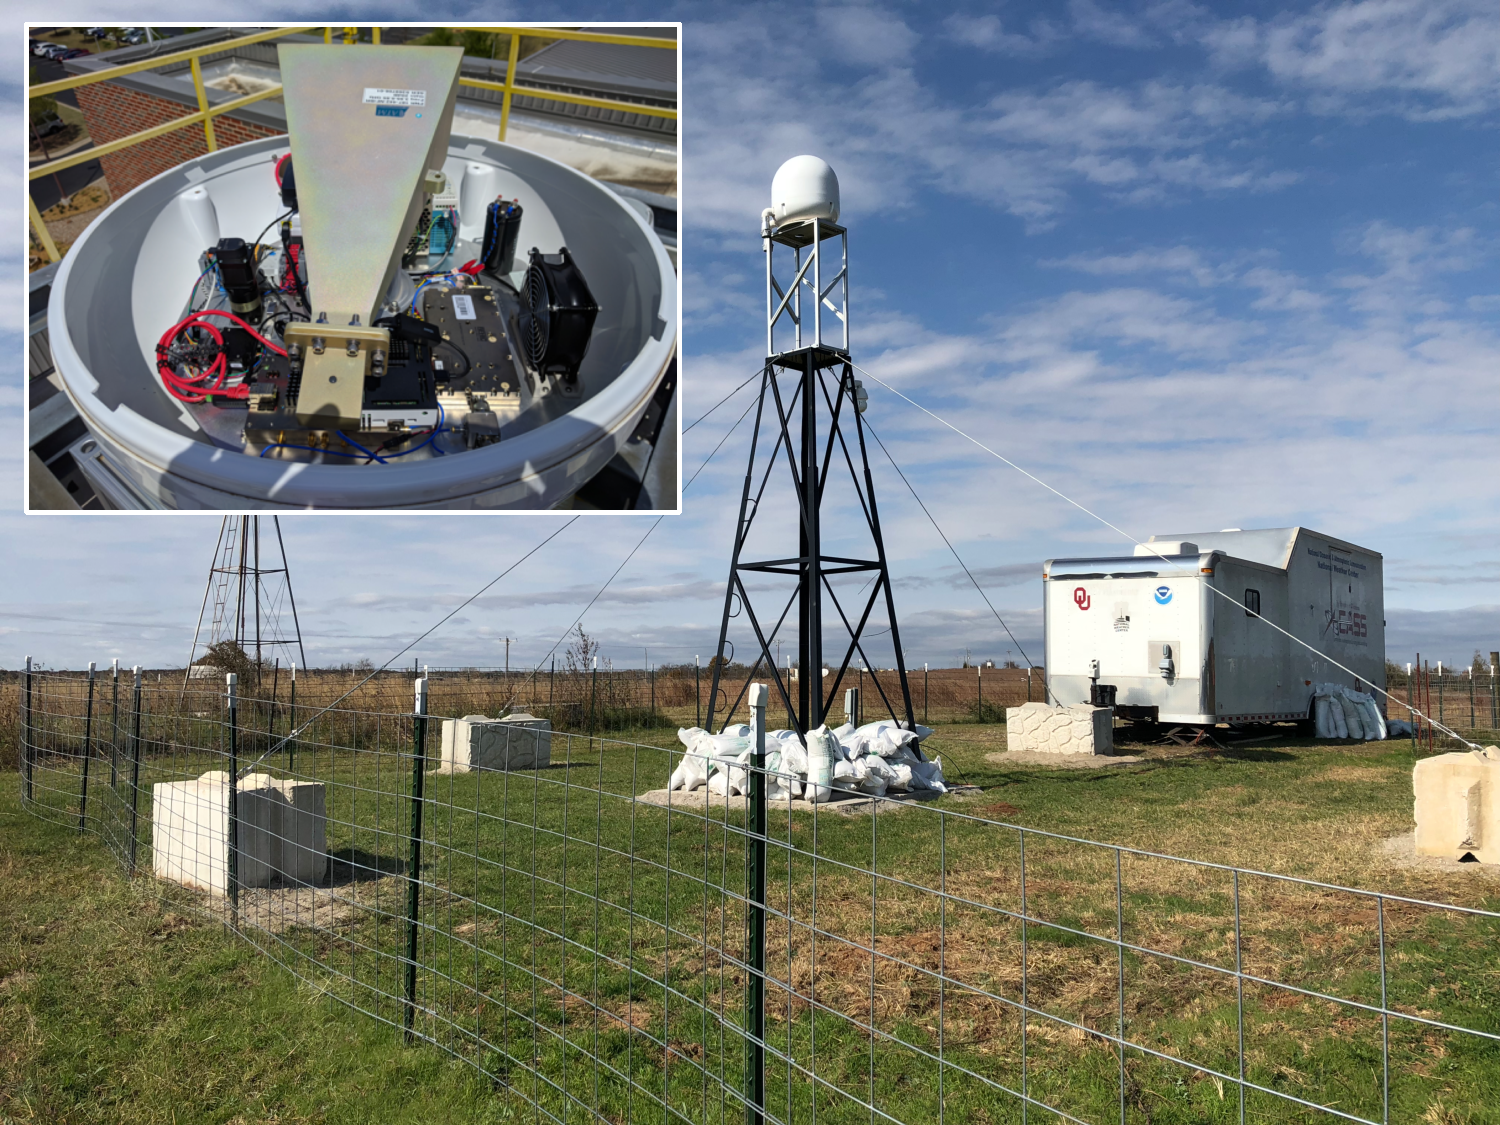
\includegraphics[angle=0, width=0.75\textwidth]{figures/GeoFenceRadarInset.pdf}
\caption{\label{fig:GeoFence} Placeholder: Picture of the GeoFence Radar mounted on a tower at KAEFS with an inset picture showing the radar hardware}
\end{figure}
% *******************************************************************************************

To detect targets, the team implemented an algorithm derived from a traditional Constant False-Alarm Rate (CFAR) detection algorithm. This algorithm uses radar data to estimate random noise levels and distinguish targets from noise.  While operating, the GBDAA Radar generates a stream of measurements, each pointed in the current direction of the radar as it spins. Once the radar completes a full circle, the receiver has assembled a Plan Position Indicator (PPI). The second component of the program is our CFAR implementation, which plots detections on an image of the PPI. We were successful in running the program in real time, ideally allowing for immediate visualization of aircraft within the radar's effective range. The program also saves data from completed PPIs and periodically stores the resulting visualization for later review.  We have conducted several flight tests.  The aircraft target used was a single-engine, four-seater Piper Warrior III, a common aircraft which served as a type specimen for the light aircraft GBDAA Radar was designed to detect. This test consisted of a series of maneuvers that aimed to test the capabilities of the GBDAA Radar. We developed a flight plan which ensured that the radar could view its target at many different altitudes and ranges. 

On February 26, 2018, the flight plan began with the plane approaching the location of the radar from the Max Westheimer Airport. The the Piper Warrior III airplane then proceeded to complete two figure-eight patterns of 1-mile radius loops. The plane then ascended to 1,500 feet, completed 2 passes over the radar, and ascended to 5,000 feet. The final maneuver of the plan was to complete a loop 4 miles in radius before returning to the airport. The route of the plan can be seen in Figure 4 below with the initial figure eight in red, the passes overhead in green, and the final loop in yellow. 

Specific detections are shown in the figure below.  In particular the graph on the left depicts the behavior of the CFAR algorithm.  The figure on the right depicts a set of detections in the lower-left quadrant.  The right wedge in the left of the figure depicts strong reflections from a nearby water tower.

% *******************************************************************************************
\begin{figure}
\centering
\includegraphics[angle=0, width=0.75\textwidth]{figures/GeoFenceData.pdf}
\caption{\label{fig:GeoFenceRadarScreen} Placeholder: GeoFence Radar screen shot. \textcolor{red}{Get original file from Yeary.} Left - detection algorithm performance , Right - several detections forming a track}
\end{figure}
% *******************************************************************************************

% ===========================================================================================
\subsection{Risk Mitigation: ADS-B}
% ===========================================================================================
\begin{itemize}[leftmargin=*,labelsep=4mm]
\color{blue}
\item	Overview of ADS-B
\item	Concept of how ADS-B in will be used to deconflict the NAS
\item	Description of our system (we need to hold back because Sai will include this in his paper)
\item	Screenshot of an aircraft detection and tracking (Figure \ref{fig:ADSBScreen})
\item	Projection of aircraft path (or leave this out) (Liz comment: I would use this as an opportunity to send them to the new paper)
\end{itemize}

We used PingStation, an ADS-B receiver from uAvionix. This receiver is a dual band networkable receiver with Power over Ethernet (POE).  The PingStation detects ADS-B equipped aircraft within a 240 km (150-mile) radius. The PingStation is robust enough to be used in harsh environmental conditions and small enough to be used as a mobile asset for roaming operations. ADS-B out (ADSB transmission) contain other parameters from the aircraft like altitude, heading, speed and flight number. This information is broadcasted to ADS-B equipped ground stations.

\begin{table}[H]
\caption{\label{tab:ADSB} Place holder: ADSB specs.}
\small % Font size can be changed to match table content. Recommend 10 pt.
\centering
\begin{tabular}{ll}
\toprule
\textbf{Specification}	& \textbf{Value}\\
\midrule
Input Voltage / Power	&44-57~V / 500~mW (Power over Ethernet)\\
Size					& 4.75'' x 2.0 '' x 3.25'' (box) 9.5'' (antenna)\\
Weight					& 340 grams\\
MTL 1090~MHz			& -88~dBm\\
Dynamic Range			& -79 to 0~dBm\\
MTL 978~MHz				& -93~dBm\\
Dynamic Range			& -90 to -3~dBm\\
\bottomrule
\end{tabular}
\end{table}

Interface is Ethernet (JSON UDP)

So, data from aircraft were obtained using an ADS-B receiver. This data was then sent to a processing computer by configuring Dynamic Host Configuration Protocol (DHCP) connection between receiver and processing computer. Mapbox is a large provider of custom online maps for websites and applications, it allows developers to build applications that are flexible for visualizing geospatial data.  In our application we used Mapbox to visualize aircraft trajectories on map. Data received by processing computer is used by Mapbox. A local host connection is used to view aircraft traffic in the browser. Mapbox together with HTML (Hypertext Markup Language) enable visualization of air traffic on the map. Air traffic on the map gets updated for every two seconds. This application was implemented in Python v3.6.

% *******************************************************************************************
\begin{figure}
\centering
\includegraphics[angle=0, width=0.75\textwidth]{figures/kess5.pdf}
\caption{\label{fig:ADSBScreen} Placeholder: Screen shot of aircraft detection and tracking. \textcolor{red}{Is there a better version of this now?}}
\end{figure}
% *******************************************************************************************

%%%%%%%%%%%%%%%%%%%%%%%%%%%%%%%%%%%%%%%%%%%%%%%%%%%%%%%%%%%%%%%%%%%%%%%%%%%%%%%%%%%%%%%%%%%%%
\section{Data Processing, Distribution, and Visualization}
%%%%%%%%%%%%%%%%%%%%%%%%%%%%%%%%%%%%%%%%%%%%%%%%%%%%%%%%%%%%%%%%%%%%%%%%%%%%%%%%%%%%%%%%%%%%%

% ===========================================================================================
\subsection{Data Processing and Distribution}
% ===========================================================================================
\begin{itemize}[leftmargin=*,labelsep=4mm]
\color{blue}
\item	Discuss data processing on the copter, on the ground station computer, and on the central processing computer
\item	Discuss how data are streamed to/from the copter and ground station and data are streamed to/from the ground station and cloud and data are streamed to/from the cloud and central processing computer
\item	Show a schematic / graphic of the data flow (Figure~\ref{fig:DataFlow})
\end{itemize}

% *******************************************************************************************
\begin{figure}
\centering
\includegraphics[angle=0, width=0.85\textwidth]{figures/dataFlow.pdf}
\caption{\label{fig:DataFlow} Placeholder: Graphic depicting the data flow \textcolor{red}{Is this still correct? Can the figure be simplified?}}
\end{figure}
% *******************************************************************************************

% ===========================================================================================
\subsection{Data Visualization}
% ===========================================================================================
\begin{itemize}[leftmargin=*,labelsep=4mm]
\color{blue}
\item	Mention the real time display on the ground station
\item	Discuss the real time display on remote servers
\item	Show a screenshot of the display (Figure~\ref{fig:GroundStationScreen})
\item	Outline how computation of data visualization will be distributed
\end{itemize}

% *******************************************************************************************
\begin{figure}
\centering
\includegraphics[angle=0, width=0.5\textwidth]{figures/dontPanic.pdf}
\caption{\label{fig:GroundStationScreen} Placeholder: Screen shot of the ground station \textcolor{red}{Get from Brian Greene.}}
\end{figure}
% *******************************************************************************************

% ===========================================================================================
\subsection{Data Examples}
% ===========================================================================================
\begin{itemize}[leftmargin=*,labelsep=4mm]
\color{blue}
\item	Provide some examples of data collection from various field experiments (Liz comment: Could be an opportunity to say that we have worked in both extremes and the knowledge we gained will make it easier for us to make our system rugged enough to deal with OK extremes.)
\item	Show a skew-T log-p plot for one sounding (Figure~\ref{fig:skewT_logp})
\item	Show a time-height plot of temperature and dew-point temperature (or similar) (Figure~\ref{fig:TimeHeightPlot})
\item	Discuss the value of having such data
\end{itemize}

% *******************************************************************************************
\begin{figure}
\centering
\includegraphics[angle=0, width=0.85\textwidth]{figures/skewT.pdf}
\caption{\label{fig:skewT_logp} Placeholder: skew T log p plot. \textcolor{red}{Get revised version from Brian Greene.}}
\end{figure}
% *******************************************************************************************

% *******************************************************************************************
\begin{figure}[htb]
\centering
%\includegraphics[angle=0, width=0.48\textwidth]{figures/20171018-1018_Temperature.pdf}
%\includegraphics[angle=0, width=0.48\textwidth]{figures/20171018-1018_Mixing.pdf}
%\includegraphics[angle=0, width=0.48\textwidth]{figures/20171018-1018_Wind.pdf}
\includegraphics[angle=0, width=0.8\textwidth]{figures/WASH_fluxcap_uas_temp_vad_color.pdf}
\caption{\label{fig:TimeHeightPlot} Time-height profiles from data collected using a profiling WxUAS.\textcolor{red}{Maybe a different plot. If we use these increase the axes labels.}}
\end{figure}
% *******************************************************************************************

%%%%%%%%%%%%%%%%%%%%%%%%%%%%%%%%%%%%%%%%%%%%%%%%%%%%%%%%%%%%%%%%%%%%%%%%%%%%%%%%%%%%%%%%%%%%%
\section{Future Directions}
%%%%%%%%%%%%%%%%%%%%%%%%%%%%%%%%%%%%%%%%%%%%%%%%%%%%%%%%%%%%%%%%%%%%%%%%%%%%%%%%%%%%%%%%%%%%%
\begin{itemize}[leftmargin=*,labelsep=4mm]
\color{blue}
\item	Continue to harden and automate the system
\item	Establish a small prototype network 
\item	Continue to evaluate the value of the measurements via OSSEs
\item	Begin assimilating data into forecast models
\end{itemize}

%%%%%%%%%%%%%%%%%%%%%%%%%%%%%%%%%%%%%%%%%%%%%%%%%%%%%%%%%%%%%%%%%%%%%%%%%%%%%%%%%%%%%%%%%%%%%
\section{Conclusions}
%%%%%%%%%%%%%%%%%%%%%%%%%%%%%%%%%%%%%%%%%%%%%%%%%%%%%%%%%%%%%%%%%%%%%%%%%%%%%%%%%%%%%%%%%%%%%
\begin{itemize}[leftmargin=*,labelsep=4mm]
\color{blue}
\item	Networks of WxUAS observations could help to fill the measurement gap in the lower atmosphere
\item	The technology is available but we need to address regulatory issues (Liz comment: Good opportunity to highlight the partnership we have with the Choctaw IPP and other COA successes we have.)
\item	Data provided by such a network could have a significant impact on weather forecasts and overall situal awareness of impending weather developments
\end{itemize}

%%%%%%%%%%%%%%%%%%%%%%%%%%%%%%%%%%%%%%%%%%
\vspace{6pt} 

%%%%%%%%%%%%%%%%%%%%%%%%%%%%%%%%%%%%%%%%%%
%% optional
\supplementary{The following are available online at www.mdpi.com/link, Figure S1: title, Table S1: title, Video S1: title.}

%%%%%%%%%%%%%%%%%%%%%%%%%%%%%%%%%%%%%%%%%%
\acknowledgments{All sources of funding of the study should be disclosed. Please clearly indicate grants that you have received in support of your research work. Clearly state if you received funds for covering the costs to publish in open access.}

%%%%%%%%%%%%%%%%%%%%%%%%%%%%%%%%%%%%%%%%%%
\authorcontributions{For research articles with several authors, a short paragraph specifying their individual contributions must be provided. The following statements should be used ``X.X. and Y.Y. conceived and designed the experiments; X.X. performed the experiments; X.X. and Y.Y. analyzed the data; W.W. contributed reagents/materials/analysis tools; Y.Y. wrote the paper.'' Authorship must be limited to those who have contributed substantially to the work reported.}

%%%%%%%%%%%%%%%%%%%%%%%%%%%%%%%%%%%%%%%%%%
\conflictofinterests{Declare conflicts of interest or state ``The authors declare no conflict of interest.'' Authors must identify and declare any personal circumstances or interest that may be perceived as inappropriately influencing the representation or interpretation of reported research results. Any role of the funding sponsors in the design of the study; in the collection, analyses or interpretation of data; in the writing of the manuscript, or in the decision to publish the results must be declared in this section. If there is no role, please state ``The founding sponsors had no role in the design of the study; in the collection, analyses, or interpretation of data; in the writing of the manuscript, and in the decision to publish the results''.} 

%%%%%%%%%%%%%%%%%%%%%%%%%%%%%%%%%%%%%%%%%%
%% optional
%\abbreviations{The following abbreviations are used in this manuscript:\\
%
%\noindent MDPI: Multidisciplinary Digital Publishing Institute\\
%DOAJ: Directory of open access journals\\
%TLA: Three letter acronym\\
%LD: linear dichroism}

%%%%%%%%%%%%%%%%%%%%%%%%%%%%%%%%%%%%%%%%%%
%% optional
%\appendix
%\section{}
%The appendix is an optional section that can contain details and data supplemental to the main text. For example, explanations of experimental details that would disrupt the flow of the main text, but nonetheless remain crucial to understanding and reproducing the research shown; figures of replicates for experiments of which representative data is shown in the main text can be added here if brief, or as Supplementary data. Mathemtaical proofs of results not central to the paper can be added as an appendix.
%
%\section{}
%All appendix sections must be cited in the main text. In the appendixes, Figures, Tables, etc. should be labeled starting with `A', e.g., Figure A1, Figure A2, etc. 

%%%%%%%%%%%%%%%%%%%%%%%%%%%%%%%%%%%%%%%%%%
\bibliographystyle{mdpi}

%=====================================
% References, variant A: internal bibliography
%=====================================
%\renewcommand\bibname{References}
%\begin{thebibliography}{999}
% Reference 1
%\bibitem{ref-journal}
%Lastname, F.; Author, T. The title of the cited article. {\em Journal Abbreviation} {\bf 2008}, {\em 10}, 142-149.
% Reference 2
%\bibitem{ref-book}
%Lastname, F.F.; Author, T. The title of the cited contribution. In {\em The Book Title}; Editor, F., Meditor, A., Eds.; Publishing House: City, Country, 2007; pp. 32-58.
%\end{thebibliography}
%
%=====================================
% References, variant B: external bibliography
%=====================================
\bibliography{chilson_refs}

%%%%%%%%%%%%%%%%%%%%%%%%%%%%%%%%%%%%%%%%%%
%% optional
%\sampleavailability{Samples of the compounds ...... are available from the authors.}

%%%%%%%%%%%%%%%%%%%%%%%%%%%%%%%%%%%%%%%%%%
\end{document}

